This section will present a pedagogically interesting 
example which demonstrates several of the programs important
features.  The purpose of this chapter is neither to be 
comprehensive nor to be particularly detailed. It will instead 
give a sense of the type of analysis that can be done easily with 
this program. It will motivate the rest of the manual. further details 
and information on any of the things described below can be found in 
the appropriate sections of the manual.

David, a user of the program, was studying iron thin films 
using powder diffraction. He was particularly interested in 
measuring the shifts in diffraction peaks of a sample. To 
realize this experimentally, he capture the image of the 
standard calibration crystal Lanthanum Hexaboride (LaB6). 
Without changing the experimental parameters, he then imaged 
many samples for which he wanted to measure the shift.

The steps that are needed to do this analysis will be
described. First, we will calibrate the diffraction detector.
This is to say that we want to determine the precise 
experimental parameters that characterized the diffraction
machine when the images were captured (for example, the distance
between sample and detector, the energy of the x-rays, etc). Since 
the image of the standard calibration crystal was taken at the same
time as the images of interest, the calibration parameters inferred
from the standard crystal can be used to analyze the
rest of data.

\begin{SCfigure}[1][hbtp]
    \centering
    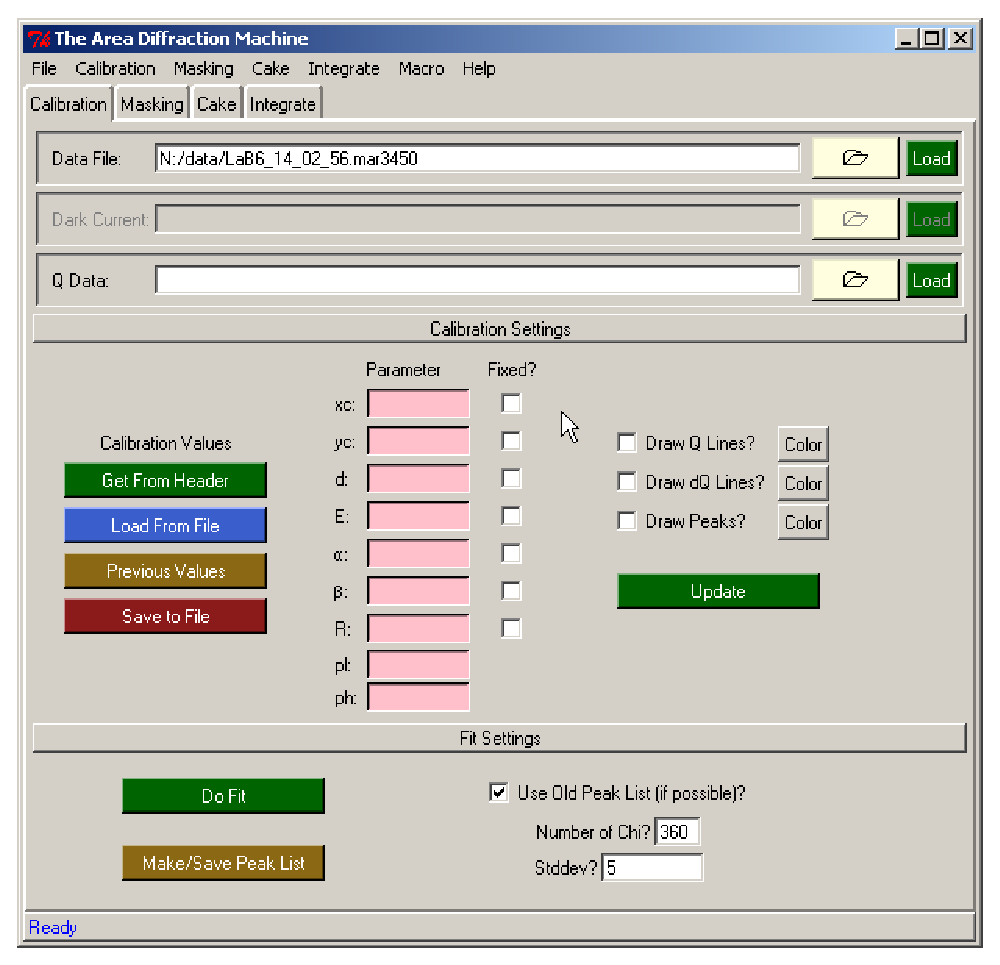
\includegraphics[scale=.75]{figures/calibration_tab.eps}
    \caption{The calibration tab.}
    \label{calibration_tab_example}
\end{SCfigure}

To perform this calibration, we first opened up the Area 
Diffraction Machine. Figure~\ref{calibration_tab_example} shows what we
are first presented with.

From the \gui{Data File} input, we load into the program the LaB6 
file. Once the file is loaded in, a new window opens up 
which shows the diffraction data. This window is shown in 
figure~\ref{diffraction_data_window_example}.

\begin{SCfigure}[1][hbtp]
    \centering
    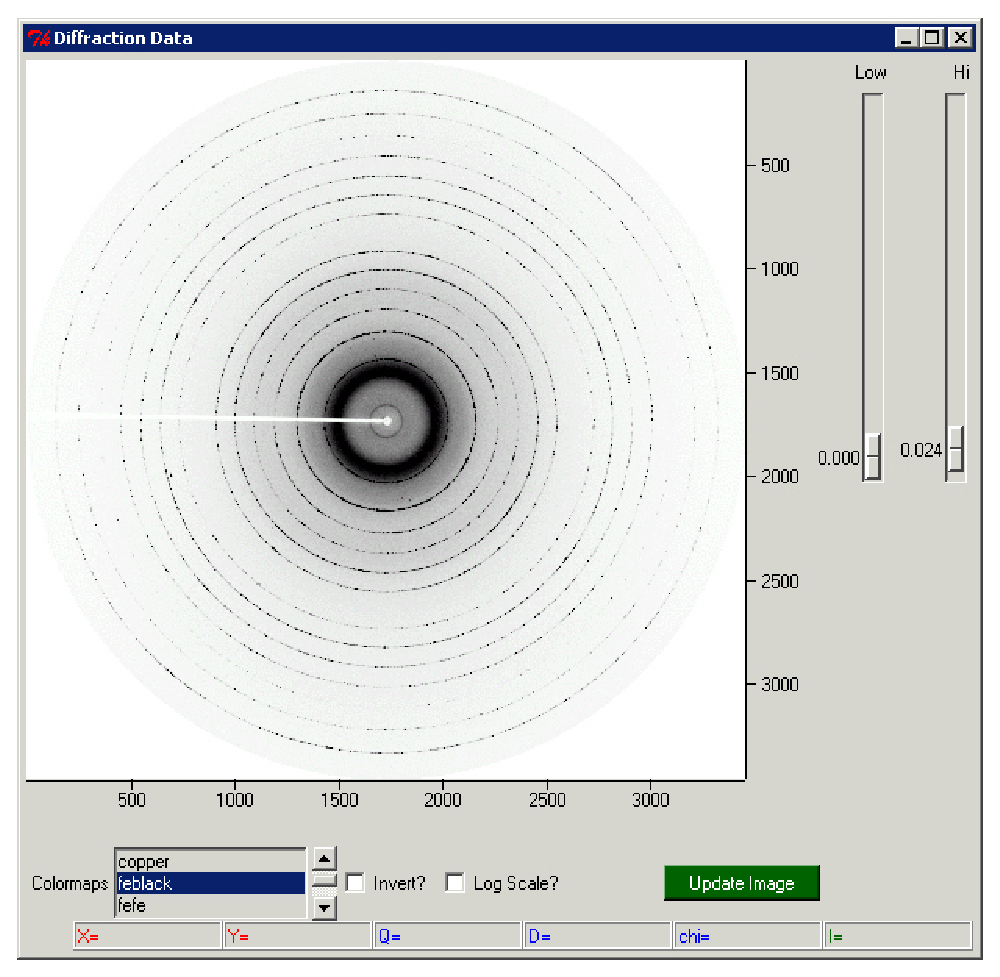
\includegraphics[scale=.75]{figures/diffraction_data_window_example.eps}
    \caption{The diffraction data window.}
    \label{diffraction_data_window_example}
\end{SCfigure}

To do the detector calibration, the program must know the 
$Q$ values associated 
with the standard crystal. Since LaB6 is so common, it is
a preset default in the program. We go into the menu bar, 
into the \gui{calibration} menu, into the \gui{Standard Q} menu, 
and then selected Lanthanum Hexaboride. This is shown
in figure~\ref{standard_q_example}.

\begin{SCfigure}[1][hbtp]
    \centering
    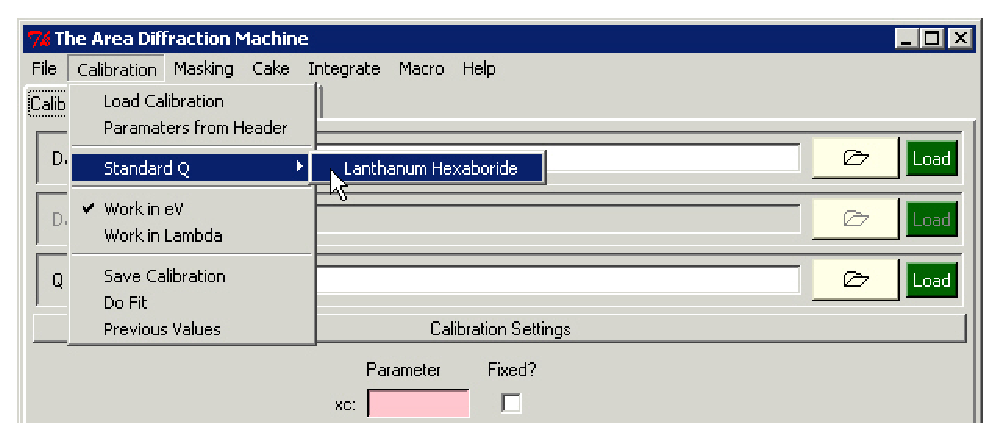
\includegraphics[scale=.75]{figures/standard_q.eps}
    \caption{Loading a standard $Q$ file.}
    \label{standard_q_example}
\end{SCfigure}

(More standard $Q$ files might be added in the future).
In order to perform image calibration, the program finally 
needs to know an initial guess at the calibration parameters. 
Although one could enter these parameters by hand, often 
times decent guesses at the experimental parameters are 
stored in the header data inside of the diffraction image. 
The program can try to find these header calibration values 
and put them into the inputs in the program. To do this, 
we could pushed the \gui{Get From Header} button. With the 
image, the $Q$ values, and an initial guess in the program, 
we are ready to do the calibration. 

But first, we want to examine how good the initial guess 
is. To do so, we can select the \gui{Draw Q Lines?}
check box on the Calibration tab. When this is selected, 
the program will draw
on top of the diffraction image red lines corresponding
to what diffraction pattern should show up on the
detector (for the given calibration parameters and $Q$
values). Figure~\ref{bad_calibration_diffraction_image}
shows what the program displays for our example.

\begin{SCfigure}[1][hbtp]
    \centering
    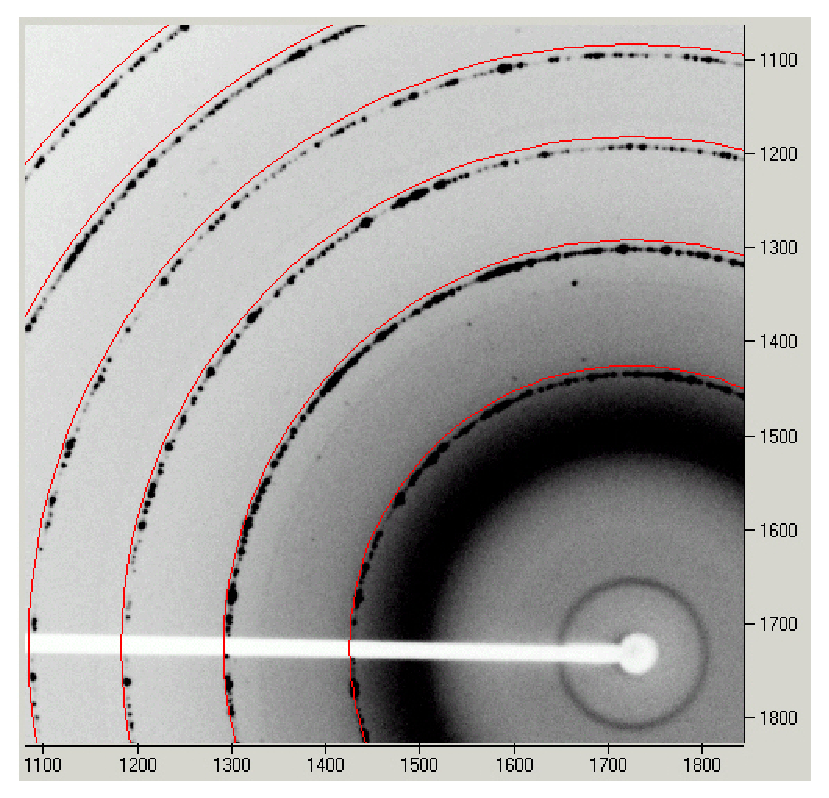
\includegraphics[scale=.75]{figures/bad_calibration_diffraction_image.eps}
    \caption{The diffraction image with constant the $Q$
    lines displayed upon it. These lines are calculated
    for the calibraiton parametesr found in the
    header of the image. They are not particuarly
    accurate.}
    \label{bad_calibration_diffraction_image}
\end{SCfigure}

Of course, our initial guess isn't
great so the red lines don't match too well with
the loaded patter. The data will look like

We can do a cake of the data. A caked plot
is a presentation of the data in a different parameter 
space.  The $x$ axis is $Q$ and the $y$ axis is $\chi$. 
Ideally, if the calibration parameters are known exactly, 
the caked data will show up as many vertical lines. 
We can cake the data by going to the cake tab. This
tab is shown in figure~\ref{cake_tab_example}.

\begin{SCfigure}[1][hbtp]
    \centering
    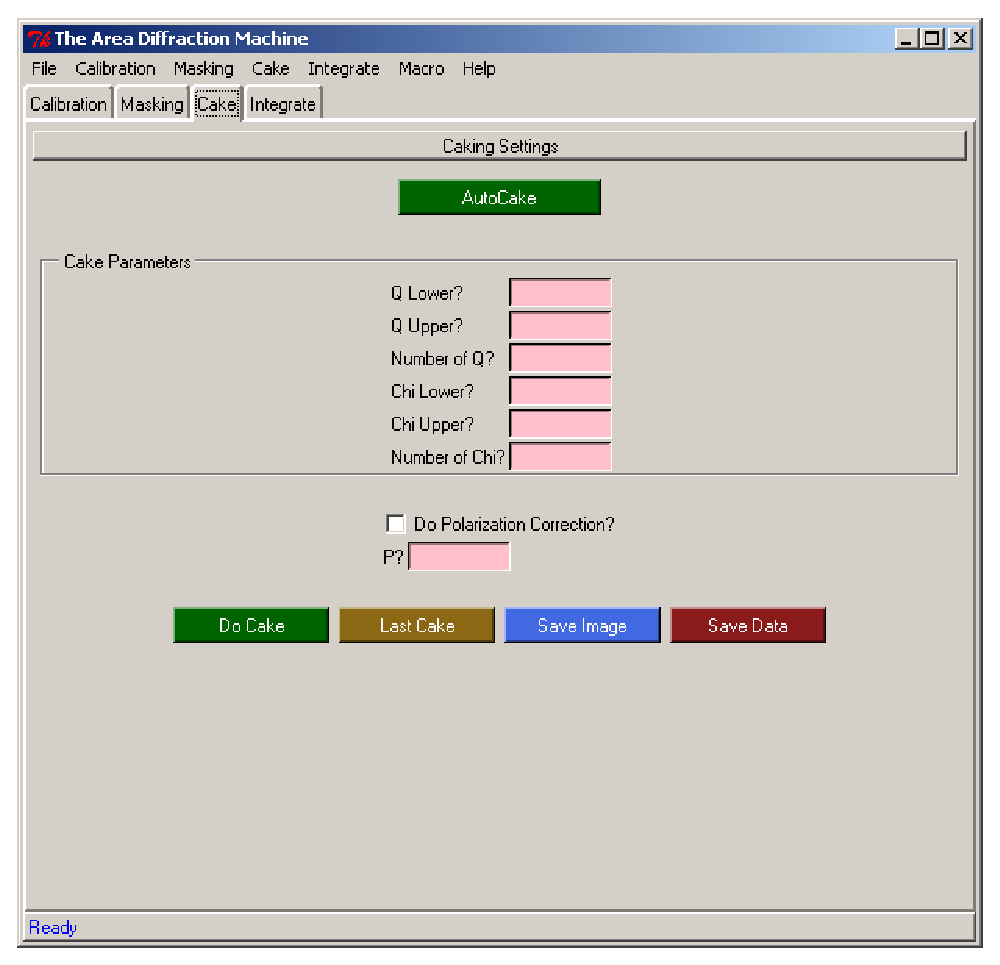
\includegraphics[scale=.75]{figures/caking_tab.eps}
    \caption{The calibration tab.}
    \label{cake_tab_example}
\end{SCfigure}

On this tab, we have to pushing the \gui{AutoCake}. 
When we do so, a new cake window opens up. 
Figure~\ref{bad_calibration_cake} shows what the 
program displays for our example.

\begin{SCfigure}[1][hbtp]
    \centering
    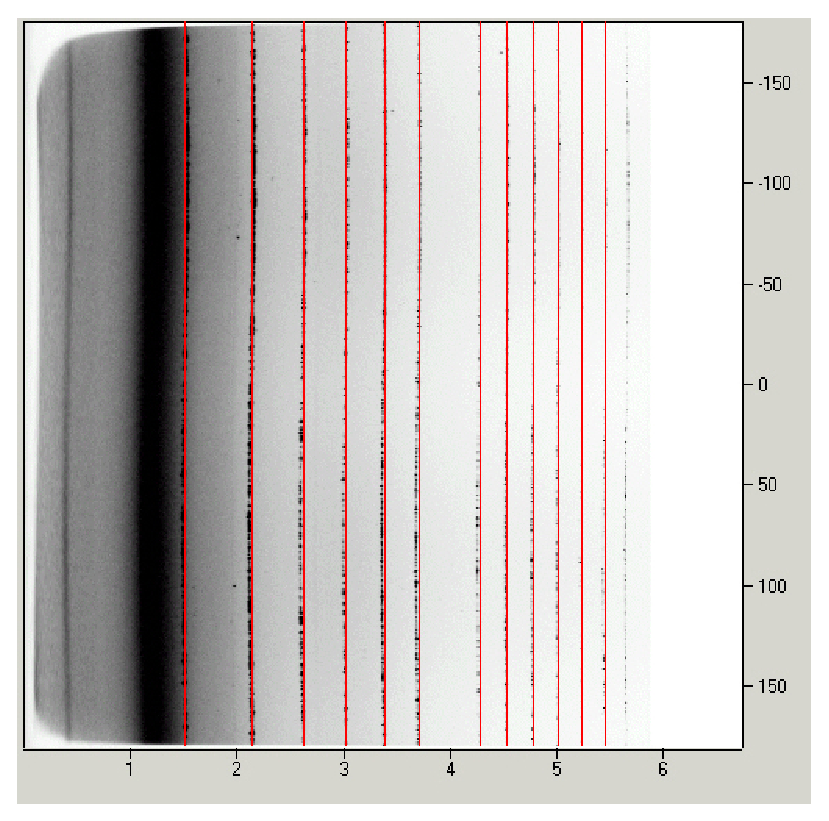
\includegraphics[scale=.75]{figures/bad_calibration_cake.eps}
    \caption{A caked plot done with the calibration parameters
    found in the header of the image. The header parameters
    are not particuarly obvious and the diffraciton peaks
    are not particuarly straight. Calibratin helps improve
    the strightness of the diffraciton peaks.}
    \label{bad_calibration_cake}
\end{SCfigure}

We see that for The caked data with the initial guess 
calibration parameters, our diffraction lines
have a systematic wiggle. It might be hard to see 
with the full image, but by zooming into just one
line we find the difference to be much more obvious.
A zoomed in range is shown in 
figure~\ref{bad_calibration_cake_zoom}.

\begin{SCfigure}[1][hbtp]
    \centering
    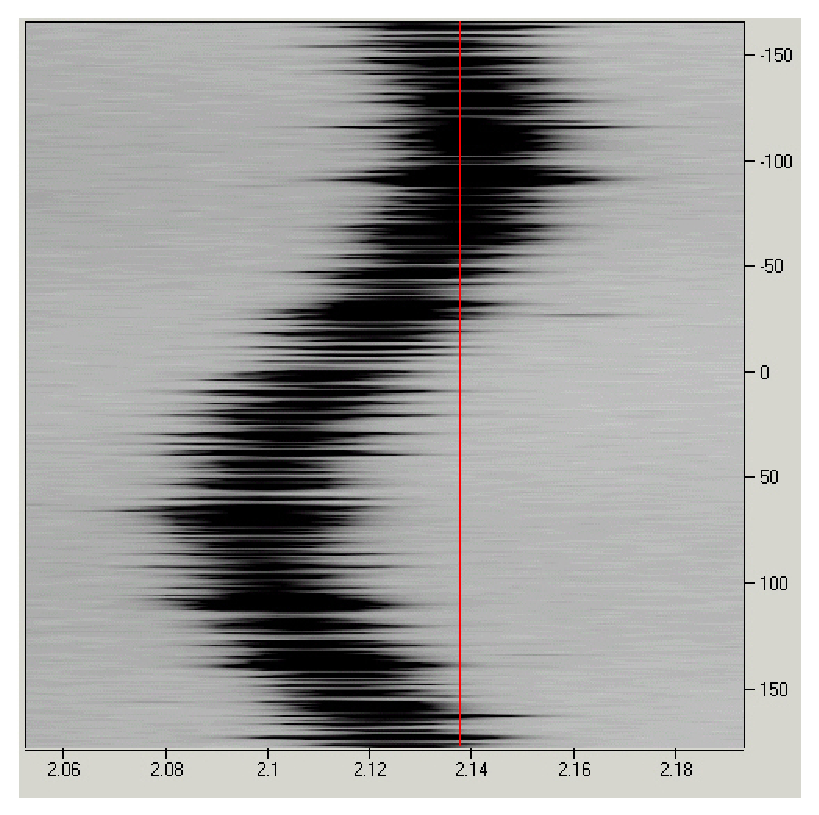
\includegraphics[scale=.75]{figures/bad_calibration_cake_zoom.eps}
    \caption{A zoom in of the cake shown in 
    figure~\ref{bad_calibration_cake}. When zoomed into 
    diffraction image, the poor calibration becomes much 
    more obvious.}
    \label{bad_calibration_cake_zoom}
\end{SCfigure}

This means that our initial guess at 
calibration parameters is not great.
We can now do the calibration. To do so, we push
the \gui{Do Fit} button on the \gui{Calibration}
tab. If the calibraiton did a good job, the constant
$Q$ lines drawn on the diffraction image move
so that they are entirely over the diffraction 
pattern. This is shown in 
figure~\ref{good_calibration_diffraction_image}.

\begin{SCfigure}[1][hbtp]
    \centering
    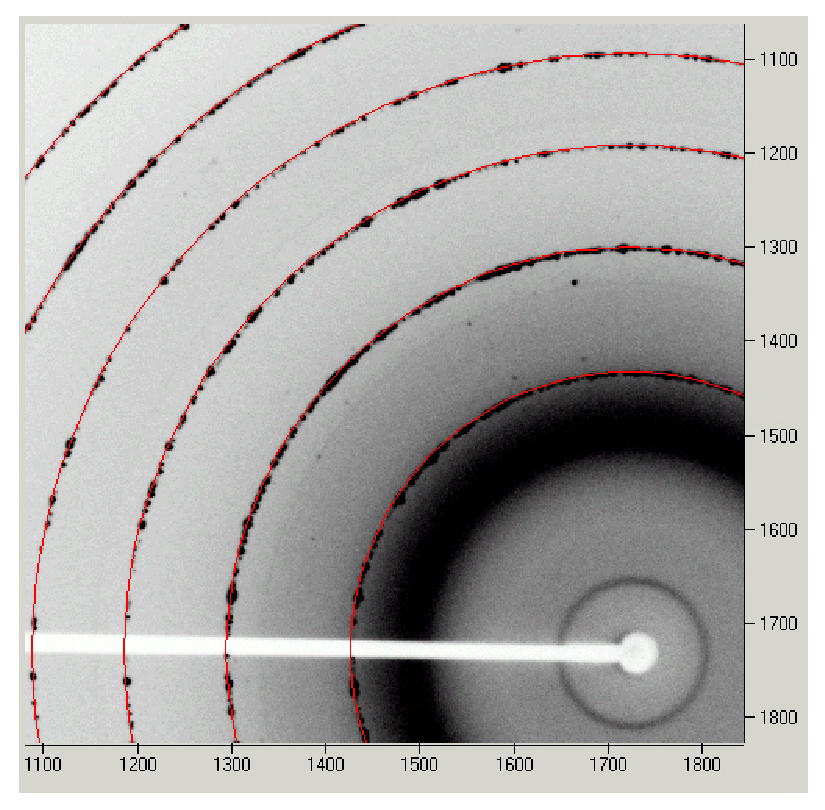
\includegraphics[scale=.75]{figures/good_calibration_diffraction_image.eps}
    \caption{The diffraction window after being calibrated. The
    constant $Q$ lines fall well on top of the diffraction 
    peaks.}
    \label{good_calibration_diffraction_image}
\end{SCfigure}

The diffraction peaks on the caked image become much straigher.
The caked window after calibraiton is shown in 
figure~\ref{good_calibration_cake}.

\begin{SCfigure}[1][hbtp]
    \centering
    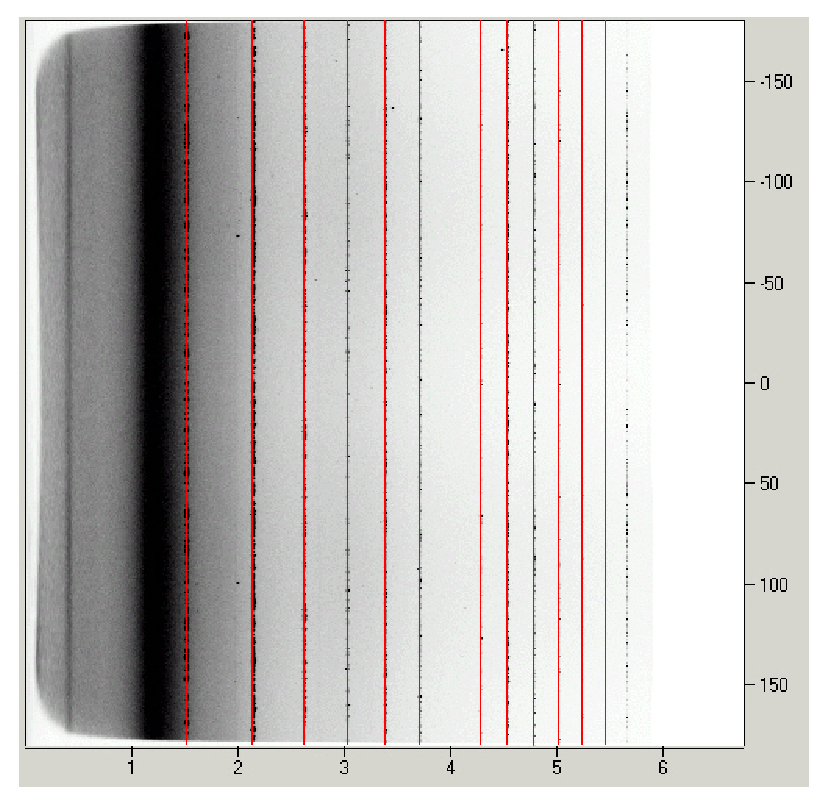
\includegraphics[scale=.75]{figures/good_calibration_cake.eps}
    \caption{The cake window after calibration.  The lines 
    are much straigher then the lines in 
    figure~\ref{bad_calibration_cake} before calibration.}
    \label{good_calibration_cake}
\end{SCfigure}

They look good even when zoomed in. A corresponding zoom in of
the caked window in shown in 
figure~\ref{good_calibration_cake_zoom}.

\begin{SCfigure}[1][hbtp]
    \centering
    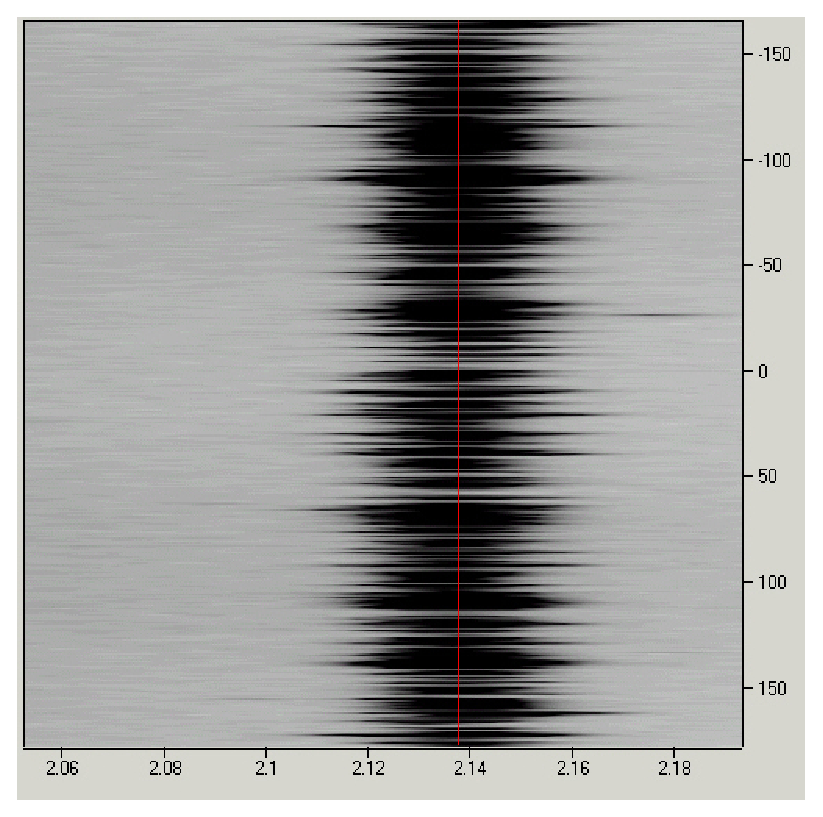
\includegraphics[scale=.75]{figures/good_calibration_cake_zoom.eps}
    \caption{A zoomed in part of figure~\ref{good_calibration_cake}. 
    Even at a large zoom in, the line remains very straight.}
    \label{good_calibration_cake_zoom}
\end{SCfigure}

After caking the calibrated data and convincing ourselves that
our calibration parameters are good, we can save the calibration
parameters to a file for later use. We can do so using the
\gui{Save to File} button on the \gui{Calibration} tab.
After selecting the location \gui{C:/Data/LaB6\_cal.dat}, the
calibration file gets saved as
\begin{lstlisting}[caption={'The Calibration Parameters File'}]
xc	1722.966078	0
yc	1724.227970	0
D	122.691351	0
E	12707.219316	0
alpha	-0.052910	0
beta	0.130553	0
rotation	-41.523477	0
pixelLength	100.000000
pixelHeight	100.000000
\end{lstlisting}

\begin{SCfigure}[1][hbtp]
    \centering
    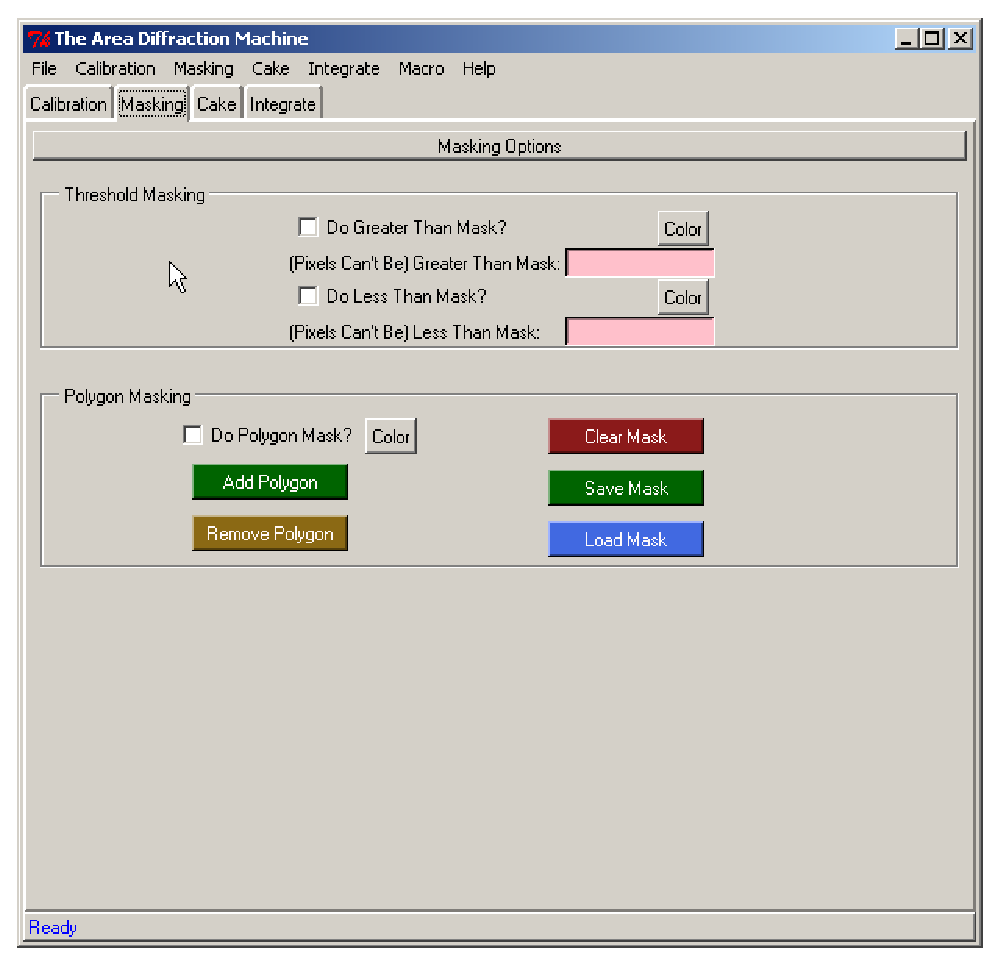
\includegraphics[scale=.75]{figures/masking_tab.eps}
    \caption{A screen shot of the pixel masking tab.}
    \label{masking_tab_example}
\end{SCfigure}

As can be seen in figure~\ref{diffraction_data_window_example},
there is a beam stop on the left side of the image which is
obstrucing part of the image. We know that none of the pixels
blocked by the beam stop contain any interesting information
so we are going to want to tell the program to ignore any pixels
blocked by the mask. We can do so with a polygon mask. All
polygon masking is done on the \gui{masking} tab. A screenshot
of this tab is shown in figure~\ref{masking_tab_example}.
We want to add a rectangular polygon mask on top of the beam
stop in the image. To do so, we push the \gui{Add Mask} button.
We then move to the diffraction image and draw the beamstop
on the image by left clicking nodes on the screen. We add the
final node by right clicking. After having drawn the polygon mask, 
our diffraction image is shown in figure~\ref{masked_beam_stop}.

\begin{SCfigure}[1][hbtp]
    \centering
    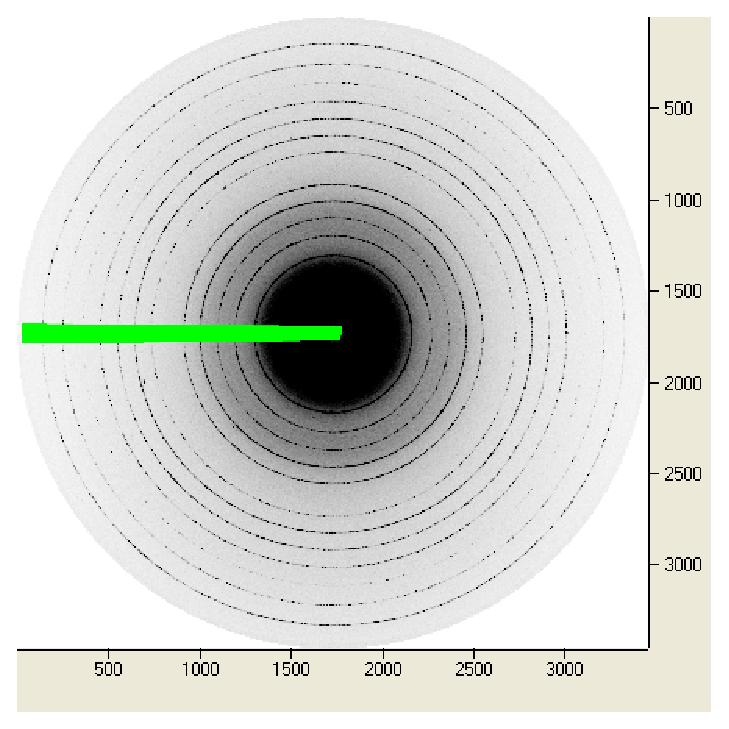
\includegraphics[scale=.75]{figures/masked_beam_stop.eps}
    \caption{}
    \label{masked_beam_stop}
\end{SCfigure}

Once we decide we are happy with our polygon mask, we can
save it to a file using the \gui{Save Mask} button.
The file gets saved out as
\begin{lstlisting}[caption={'beam\_stop\_mask.dat'}]
# Polygon(s) drawn on Mon Apr 14 00:33:12 2008
25.6749379653	1634.63771712
42.7915632754	1814.36228288
1959.85359801	1857.15384615
1959.85359801	1626.07940447
\end{lstlisting}
We can then load in this mask when we do the rest of
our analysis. The mask will make sure that none of the
the pixels within the beam stop are used for any subsequent
analysis.

Now, we are going to want to perform an intensity integration 
of the rest of our data. We can use the intensity
integrate data to look for peaks in the data.
The steps for doing the rest of
this analysis are as follows. Load in particular file we
are interested in. Load in these calibration parameters
using the \gui{Load From File} button on the \gui{Calibration}
tab.\footnote{If you just did the calibration, the 
parameters should already be in the inputs. The point is
just that you could load the parameters into the program
if you were, say, to open the program at some later point
in time.}. Next, we can load in our previously recorded
beam stop mask using the \gui{Load Mask} button on the
\gui{Masking} tab. With everything loaded into the program, 
we can perform a $Q$ integration by going to the 
\gui{Integrate} tab. The integration tab is shown in 
figure~\ref{integration_tab_example}

\begin{SCfigure}[1][hbtp]
    \centering
    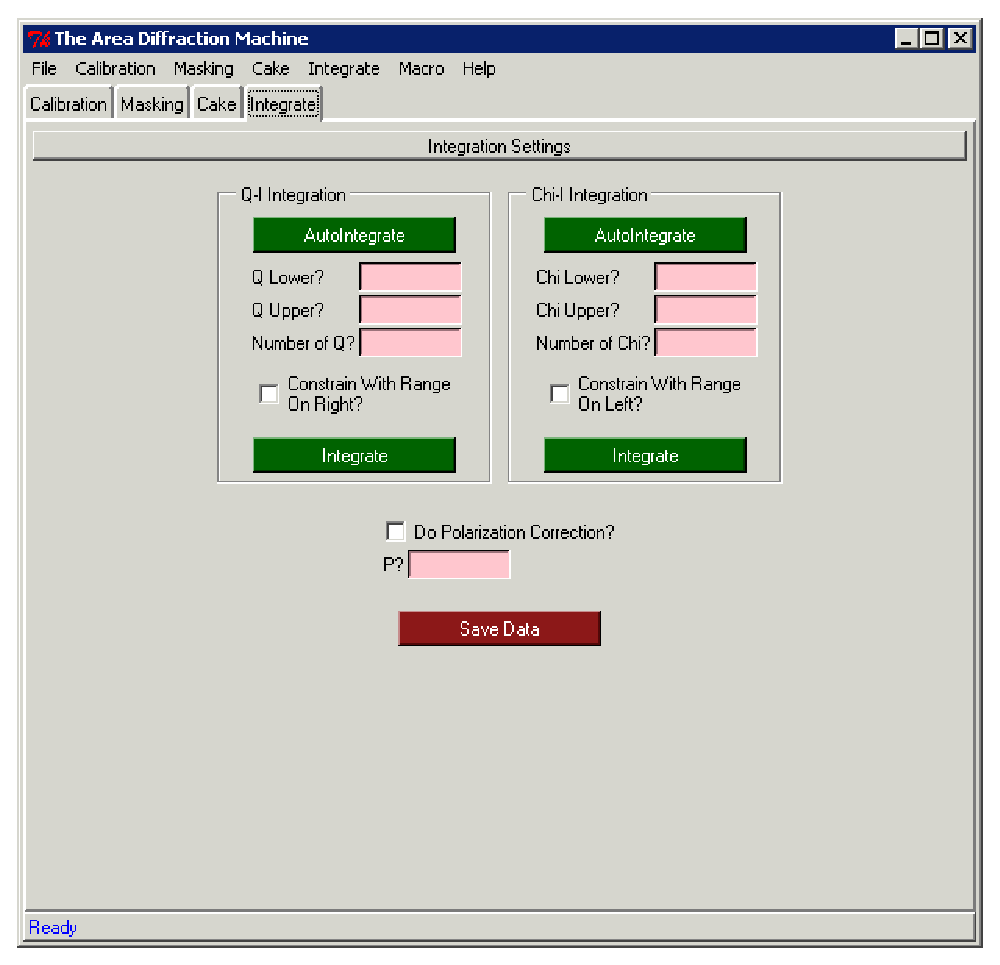
\includegraphics[scale=.75]{figures/integration_tab.eps}
    \caption{The integration tab.}
    \label{integration_tab_example}
\end{SCfigure}

We set the range of the $Q$ integration by setting
\gui{Q Lower?} to 0 and \gui{Q Upper?} to 5. We
then set the precision of the integration, or the
bin size, by setting the \gui{Number of Q?} input
to 300. Finally, we push the left \gui{Integrate}
button and a window showing the diffraction data
opens. For a particular iron sample, this window
is shown in figure~\ref{iron_intensity}.

\begin{SCfigure}[1][hbtp]
    \centering
    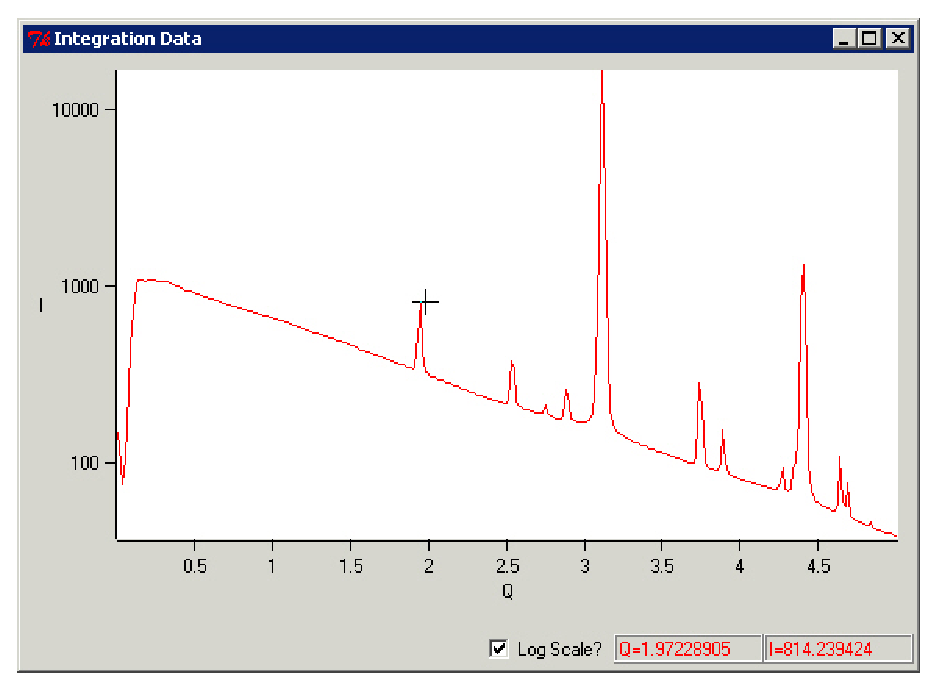
\includegraphics[scale=.75]{figures/iron_intensity.eps}
    \caption{The intensity integration window for 
    a particular iron sample.}
    \label{iron_intensity}
\end{SCfigure}

We can save this data to a file with the \gui{Save Data}
button on the \gui{Integration} tab. This data is
saved out as two column ASCII.
After doing this for all the different files that
we have, we can load all the data into another program,
such as Microsoft Excel, and compare the peaks.

But if there are a lot of files to analyze, this whole
process can be very time consuming. Instead of doing 
this analysis by hand, we can automate the process by
writing a macro to analyze all the files one at a 
time. First, we put all of our data into \macroline{C:/Data/}.
The macro that we can run is
\begin{lstlisting}[caption={'A macro to automate the 
    analysis'}]
Data File:
	C:/Data/
Load From File
    C:/Data/LaB6_cal.dat
Load Mask
    C:/Data/beam_stop_mask.dat
Integrate Q Lower?
	0
Integrate Q Upper?
	5
Integrate Number of Q?
	300
Integrate Q-I
Save Integration Data
    PATHNAME/FILENAME_int.dat
\end{lstlisting}
The first command loads into the program all of the
diffraction files in the folder \macroline{C:/Data/}
one at a time and runs the rest of the analysis on
that particular file. The program then loads in
the calibration file that we saved earlier and sets the
integration bounds. Then the progarm loads in the
beam stop mask. Then, the program does a 
$Q$ vs intensity integration and saves the intensity
integrated data to a file. The PATHNAME keyword gets
repalced with teh path leading up to the particular 
file and the FILENAME keyword gets replaced with 
the particular file's name. For example, the file
\macroline{FeL2\_d070.mar3450} in
the folder \macroline{C:/Data/} would
be replaced with
\macroline{C:/Data/FeL2\_d070\_int.dat}
This command will let us save out of our intesnity
integrated data next to the corresponding diffraction
file with a useful filename.

After we run this macro, all of our data will 
be saved out into text files. We can, for
example, open the files in Excel and plot
the different diffraction patterns on the same
graph. If we did this, we would obtain a plot
that looked something like the graph shown
in figure~\ref{excel_peak_shift}.

\begin{SCfigure}[1][hbtp]
    \centering
    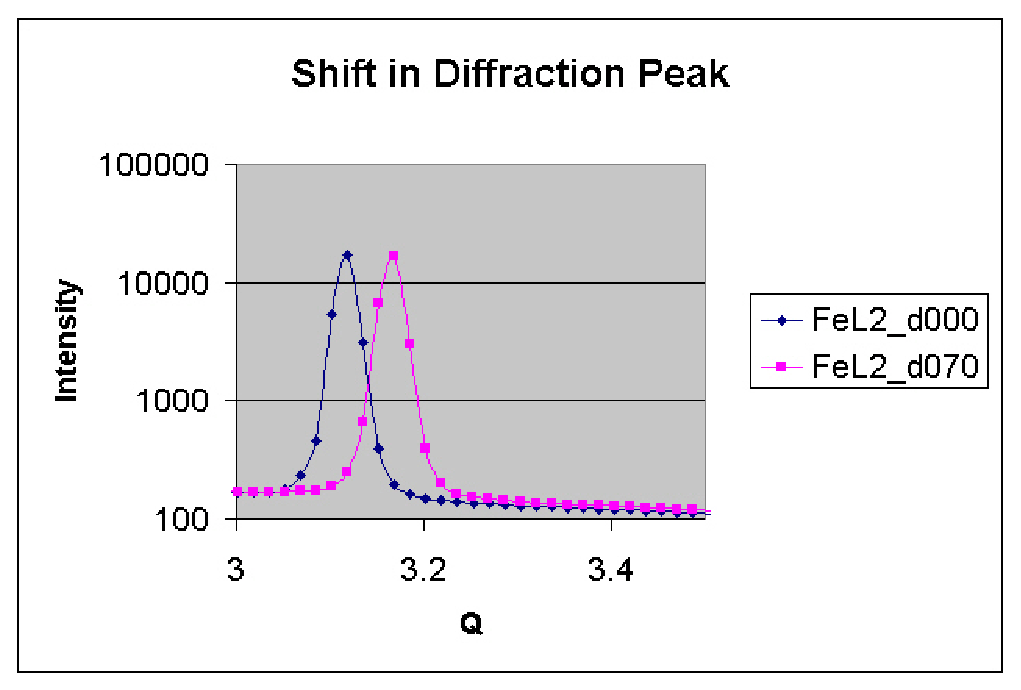
\includegraphics[scale=.5]{figures/excel_peak_shift.eps}
    \caption{An example of what the shift in peaks might
    look like when two diffraction patterns were plotted
    in Excel on top of one another.}
    \label{excel_peak_shift}
\end{SCfigure}


